%------------------------------------------------------------------------------
% Beginning of trunki.tex
%------------------------------------------------------------------------------
\documentclass{amsart}

%     If your article includes graphics, uncomment this command.
\usepackage{graphicx}

\numberwithin{equation}{section}

%    Absolute value notation
\newcommand{\abs}[1]{\lvert#1\rvert}

%    Blank box placeholder for figures (to avoid requiring any
%    particular graphics capabilities for printing this document).
\newcommand{\blankbox}[2]{%
  \parbox{\columnwidth}{\centering
%    Set fboxsep to 0 so that the actual size of the box will match the
%    given measurements more closely.
    \setlength{\fboxsep}{0pt}%
    \fbox{\raisebox{0pt}[#2]{\hspace{#1}}}%
  }%
}

%    Eliott's added commands
\newcommand{\bC}{\mathbf{C}}
\newcommand{\bD}{\boldsymbol{D}}
\newcommand{\bG}{\boldsymbol{G}}
\newcommand{\bK}{\mathbf{K}}
\newcommand{\bM}{\mathbf{M}}
\newcommand{\br}{\boldsymbol{r}}
\newcommand{\bq}{\boldsymbol{q}}
\newcommand{\bQ}{\boldsymbol{Q}}
\newcommand{\bv}{\boldsymbol{v}}
\newcommand{\bV}{\mathbf{V}}

\begin{document}

\title{Drubble}

%    Information for first author
\author{Eliott Radcliffe}
%    Address of record for the research reported here
%\address{1513 Constitution Ave NE \#3, Washington, DC 20002}
%    Current address
\curraddr{1513 Constitution Ave NE \#3, Washington, DC 20002}
\email{radcli14@gmail.com}

%\date{January 1, 2001 and, in revised form, June 22, 2001.}

\keywords{Dynamics}

\begin{abstract}
asdf
\end{abstract}

\maketitle

\section{Introduction}
asdf

\section{The History of Drubble}
A game we used to play while drinking in college.

\subsection{Single Player Drubblei}
Throw it up, bounce it on the stool, try to keep it bouncing.

\subsection{Two Player Drubble}
First person throws it, second person tries to bounce it as far as they can on the stool.

\subsection{Three Player Drubble}
First person throws it, second person bounces it to the third person, who bounces it to the first person who has run behind them.

\section{Dynamics Model}
\begin{figure}
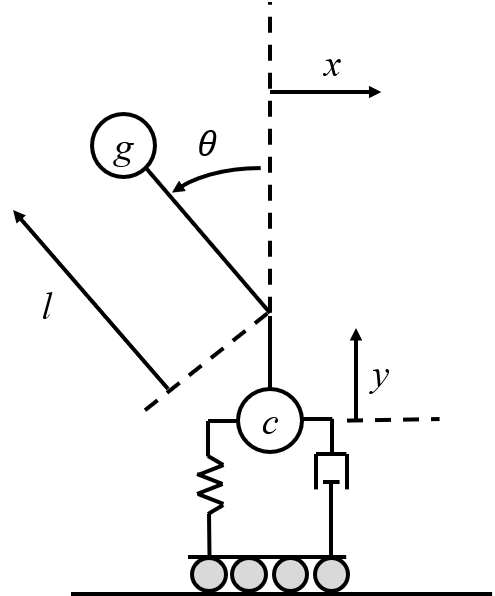
\includegraphics[width=3in]{diagram.png}
\end{figure}

The generalized coordinate vector is
\begin{equation}
\bq = \left(x,y,l,\theta\right)^T
\end{equation}
Person is a point mass that can translate in two directions, their position is
\begin{equation}
\br_c = \begin{bmatrix} x \\ y \end{bmatrix}
\end{equation}
and their velocity is
\begin{equation}
%\dot\br_c 
\bv_c = \begin{bmatrix} \dot x \\ \dot y \end{bmatrix} ,
\end{equation}
and the matrix containing derivatives of $\dot\br_c$ with respect to $\bq$ is
\begin{equation}
\bV_c = \begin{bmatrix} 1 & 0 & 0 & 0 \\ 0 & 1 & 0 & 0 \end{bmatrix} .
\end{equation}
The position of the stool is
\begin{equation}
\br_g = \begin{bmatrix} x-l\sin\theta \\ y+a+l\cos\theta \end{bmatrix}
\end{equation}
and its velocity is
\begin{equation}
%\dot\br_g 
\bv_g = \begin{bmatrix} 
\dot x -\dot l \sin\theta - l\dot\theta\cos\theta \\ 
\dot y +\dot l \cos\theta - l\dot\theta\sin\theta 
\end{bmatrix} , 
\end{equation}
and the matrix containing derivatives of $\dot\br_g$ with respect to $\bq$ is
\begin{equation}
\bV_g = \begin{bmatrix} 
1 & 0 & -\sin\theta & -l\cos\theta \\ 
0 & 1 & \cos\theta & -l\sin\theta 
\end{bmatrix} .
\end{equation}

Lagranges method used to define equations of motion
\begin{equation}
\frac{d}{dt}\left( \frac{\partial L}{\partial\dot\bq} \right)-\frac{\partial L}{\partial\bq} = \bQ
\end{equation}
where $L=T-V$. Kinetic energy is
\begin{multline}
T = \frac{1}{2} \dot\bq^T \bM \dot\bq \\ 
= \frac{1}{2}\bigg( \
(m_c+m_g)\dot x^2 + (m_c+m_g)\dot y^2 + m_g\dot l^2 + m_gl^2\dot\theta^2 \\ 
- 2m_g\dot x\dot l\sin\theta - 2m_g\dot x\dot\theta l\cos\theta %\\
+ 2m_g\dot y\dot l\cos\theta - 2m_g\dot y\dot\theta l\sin\theta 
\bigg)
\end{multline}
where the mass matrix
\begin{equation}
\bM = m_c \bV_c^T\bV_c + m_g \bV_g^T\bV_g = 
\begin{bmatrix}
m_c+m_g & 0 & -m_g\sin\theta & -m_gl\cos\theta \\
0 & m_c+m_g & m_g\cos\theta & -m_gl\sin\theta \\
-m_g\sin\theta & m_g\cos\theta & m_g & 0 \\
-m_gl\cos\theta & -m_gl\sin\theta & 0 & m_gl^2
\end{bmatrix}
.
\end{equation}
These can be used to derive 
\begin{equation}
\frac{d}{dt}\left( \frac{\partial T}{\partial\dot\bq} \right) = \bM\ddot\bq + \dot\bM\dot\bq
\end{equation}
where 
\begin{equation}
\dot\bM = m_g\begin{bmatrix}
0 & 0 & -\dot\theta\cos\theta & -\dot l\cos\theta + l\dot\theta\sin\theta \\
0 & 0 & -\dot\theta\sin\theta & -\dot l\sin\theta - l\dot\theta\cos\theta \\
-\dot\theta\cos\theta & -\dot\theta\sin\theta & 0 & 0 \\
-\dot l\cos\theta + l\dot\theta\sin\theta & -\dot l\sin\theta - l\dot\theta\cos\theta & 0 & 2l\dot l
\end{bmatrix}
\end{equation}
\begin{equation}
\dot\bM\dot\bq = m_g\begin{bmatrix}
-2\dot l\dot\theta\cos\theta + l\dot\theta^2\sin\theta \\
-2\dot l\dot\theta\sin\theta - l\dot\theta^2\cos\theta \\
-\dot x\dot\theta\cos\theta - \dot y\dot\theta\sin\theta \\
-\dot x\dot l\cos\theta + \dot xl\dot\theta\sin\theta -\dot y\dot l\sin\theta -\dot yl\dot\theta\cos\theta 
\end{bmatrix}
\end{equation}
%\end{equation}
The derivatives
\begin{multline}
\frac{\partial T}{\partial\bq} = \frac{1}{2} m_g \begin{bmatrix}
0 \\ 0 \\ \dot\bq^T \bigg( [\partial\bV_g^T / \partial l]^T \bV_g + \bV_g^T [\partial \bV_g / \partial l] \bigg) \\ 
\dot\bq^T \bigg( [\partial\bV_g^T / \partial\theta]^T\bV_g + \bV_g^T [\partial\bV_g / \partial\theta ] \bigg)
\end{bmatrix} \dot\bq \\
=m_g\begin{bmatrix}
0 \\ 0 \\ 
-\dot x\dot\theta\cos\theta - \dot y\dot\theta\sin\theta \\
-\dot x \dot l\cos\theta + \dot x \dot\theta l\sin\theta - \dot y\dot l\sin\theta - \dot y\dot\theta l \cos\theta
\end{bmatrix}
\end{multline}
where
\begin{equation}
\frac{\partial\bV_g}{\partial l} = \begin{bmatrix}
0 & 0 & 0 & -\cos\theta \\
0 & 0 & 0 & -\sin\theta \\
\end{bmatrix}
\end{equation}
and
\begin{equation}
[\partial\bV_g^T / \partial l]^T\bV_g = \begin{bmatrix}
0 & 0 & 0 & 0 \\
0 & 0 & 0 & 0 \\
0 & 0 & 0 & 0 \\
-\cos\theta & -\sin\theta & 0 & l
\end{bmatrix}
\end{equation}
and
\begin{equation}
\frac{\partial\bV_g}{\partial\theta} = \begin{bmatrix}
0 & 0 & -\cos\theta & l\sin\theta \\
0 & 0 & -\sin\theta & -l\cos\theta
\end{bmatrix} .
\end{equation}
Define
\begin{equation}
\bD = 
\dot\bM\dot\bq - \frac{\partial T}{\partial \bq} = \begin{bmatrix}
-2\dot l\dot\theta\cos\theta + l\dot\theta^2\sin\theta \\
-2\dot l\dot\theta\sin\theta - l\dot\theta^2\cos\theta \\ 
0 \\ 0 
\end{bmatrix}
\end{equation}

Potential energy is
\begin{equation}
V = \frac{1}{2}k_y(y-y_0)^2 + 
\frac{1}{2}k_l(l-l_0)^2 + 
\frac{1}{2}k_\theta\theta^2 + 
g(m_c+m_g)y + gm_gl\cos\theta
\end{equation}
and derivatives
\begin{equation}
\frac{\partial V}{\partial\bq} = \bK\bq - \bK\bq_0 + \bG
\end{equation}
where
\begin{equation}
\bK = \textnormal{diag}(0,k_y,k_l,k_\theta)
\end{equation}
and
\begin{equation}
\bG = 
g\begin{bmatrix}
0 \\ m_c+m_g \\ m_g\cos\theta \\ -m_gl\sin\theta
\end{bmatrix}
\end{equation}
and $\partial V / \partial\dot\bq = (0,0,0,0)^T$.

Combining the above gives the equations of motion
\begin{equation}
\bM\ddot\bq = - \bC\dot\bq - \bK\bq + \bK\bq_0 -\bD - \bG +\bQ
\end{equation}

\section{Application}
Built the app using ...

\subsection{Controls}
Left hand controls stool, right hand controls person.

\section{Conclusions}
Made a dollar.

\bibliographystyle{amsplain}
\begin{thebibliography}{10}

\bibitem{Greenwood} D. T. Greenwood, ``Principles of Dynamics''

\end{thebibliography}

\end{document}

%------------------------------------------------------------------------------
% End of journal.tex
%------------------------------------------------------------------------------
